\label{section:azure:datalake}
\label{todo:datalake_description}
\textit{Azure DataLake Gen2} is a cloud storage service.
It is possible to store and retrieve files of any format and up to 8TB size.

\subsubsection{Blob storage}
    Files are stored under a Blob storage format, which is an Azure-developed format optimized for storing massive amounts of unstructured data \cite{bib:azure:datalake:intro_to_blob_storage}.
    
    Blob storage offers three types of resources:
        \begin{itemize}
            \item The storage account.
            \item A container in the storage account.
            \item A blob in a container.
        \end{itemize}

    Figure \ref{fig:azure:datalake:resources_relationship} shows the relationship between these resources.
    Files are memorized in a blob, i.e, a particular distributed storage format which can contain pieces of multiple files.
    
    \begin{figure}
        \centering
        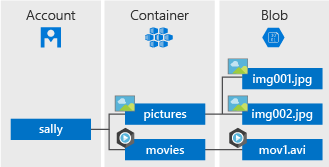
\includegraphics[width=.5\textwidth]{res/azure/datalake/blob.png}
        \caption{Relationship between DataLake resources.}
        \label{fig:azure:datalake:resources_relationship}
    \end{figure}

    Permissions can be set at container level or at file level.
    Under each container it is possible to upload or download files, or to organize them into sub-folders.
    
    Data can be accessed through HTTP or HTTPS.
    It is also possible to mount the Blob storage as a file system through the \texttt{abfss}\footnote{
        \textit{Azure Blob File System}. The last \texttt{s} means the protocol is \textit{Secure}, i.e., it requires SSL authentication.
    } protocol.
    \paragraph{Blob types}
        Azure Storage supports three types of blobs \cite{bib:azure:datalake:intro_to_blob_storage}:
            \begin{itemize}
                \item Block blobs store text and binary data, up to about 4.7 TB. Block blobs are made up of blocks of data that can be managed individually.
                \item Append blobs are made up of blocks like block blobs, but are optimized for append operations. Append blobs are ideal for scenarios such as logging data from virtual machines.
                \item Page blobs store random access files up to 8 TB in size. Page blobs that store the virtual hard drive files serve as disks for Azure virtual machines.
            \end{itemize}
            
        All files used by Databricks, given their relatively small size (a few MB per file) are stored as block blobs.

